\documentclass[11pt]{article}
\usepackage{freerbmt09}

\usepackage[pdftex]{graphicx}
%\usepackage{graphics}
%\usepackage{rotating}
%\usepackage{ucs}

\usepackage[utf8x]{inputenc}
\usepackage{times}
\usepackage{natbib}
\usepackage{url}
\usepackage{latexsym}

\usepackage[small,bf]{caption}

\newtheorem{cs}{Case Study}

\title{Leveraging Service-Oriented Architectures through efficient and scalable Rule-Based Machine Translation services}

\author{Pasquale Minervini\\
  Dipartimento di Informatica\\
  Università degli Studi di Bari\\
  Via E. Orabona 4, 70125 Bari, Italy\\
  {\tt p.minervini@gmail.com}}

\date{}

\begin{document}

\maketitle

\begin{abstract}
Service Oriented Architecture (SOA) is a paradigm for organizing and utilizing distributed services that may be under the  control of different ownership domains and implemented using various technology stacks. In some contexts, an organization using an IT infrastructure implementing the SOA paradigm can take a great benefit from the integration, in its business processes, of efficient Machine Translation services to overcome language barriers. This paper describes the architecture used to develop a Machine Translation service that is efficient, scalable and easy to integrate in new and existing business processes; our service relies on Apertium, a Free/Open-Source Rule-Based Machine Translation platform.
\end{abstract}


\section{Introduction}

Service Oriented Architecture is an architectural paradigm providing a set of principles of governing concepts used during phases of systems development and integration. In such an architecture, functionalities are packaged as interoperable, loosely coupled services that may be used to build infrastructures enabling those with needs (consumers) and those with capabilities (providers) to interact across different domains of technology and ownership.

Several new trends in the computer industry rely upon SOA as the enabling foundation, including the automation of Business Process Management (BPM) and the multitude of new architecture and design patterns generally referred to as Web 2.0~\citep{web20}.\\

In some contexts, an organization using an IT infrastructure implementing the SOA paradigm can take a great benefit from the integration, in its business processes, of an efficient Machine Translation service to overcome language barriers; for instance, it could be integrated in collaborative enviroments where people, who have no language in common, attempt to communicate with each other, or in knowledge extraction processes, where data is not available in a language that can be comprehended by the domain experts or the knowledge extraction tools beign used.

\begin{cs}{\bf - UMLS$^{\mbox{\small\textregistered}}$ concepts identification in non-English medical documents:}
MetaMap~\citep{metamap} is an application that allows mapping text to UMLS$^{\mbox{\small\textregistered}}$ Metathesaurus$^{\mbox{\small\textregistered}}$\footnote{The UMLS$^{\mbox{\small\textregistered}}$ Metathesaurus$^{\mbox{\small\textregistered}}$~\citep{umls} provides a representation of biomedical knowledge consisting of concepts classified by semantic type and both hierarchical and non-hierarchical relationships among the concepts.} concepts, which have proved to be useful for many applications, including decision support systems, management of patient records, information retrieval and data mining within the biomedical domain.


\begin{figure}[!ht]
\begin{center}
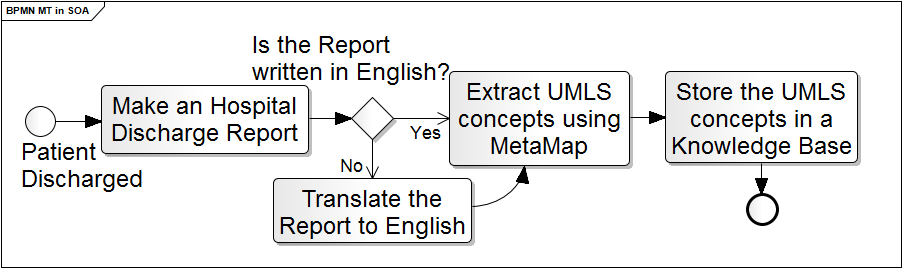
\includegraphics[width=7.75cm]{mtsoa}
\end{center}
\caption{Representation of a business process in which a clinical document, if written in a language different than English, is fist translated to English and then processed using MetaMap to extract UMLS$^{\mbox{\small\textregistered}}$ concepts.}
\label{fig:mtsoa}
\end{figure}

Currently MetaMap is only available for English free text, which makes it difficult the use of UMLS$^{\mbox{\small\textregistered}}$ Metathesaurus$^{\mbox{\small\textregistered}}$ to represent concepts from biomedical texts written in languages other than English. A possible way to overcome this limitation consists in using Machine Translation techniques (possibly with dictionaries, translation rules, lexical selection techniques etc. specific for the biomedical domain) to translate the free text from its original language to English, and then process it as in Figure \ref{fig:mtsoa}. This approach is also discussed in \shortcite{metamapes}.
\end{cs}

\begin{cs}{\bf - Supporting creation of user-generated content:}
Wikipedia is an online, multilingual, volunteer-edited encyclopedia. ``There are currently 262 language editions of Wikipedia; of these, 24 have over 100,000 articles and 81 have over 1,000 articles''~\citep{wikipedia}. Although access to technology is also an important factor, the number of available articles in a particular language's Wikipedia corresponds somewhat to the number of available speakers of that language.

In many cases, closely related languages are mutually intelligible~\citep{tyers09a}, and even a prototype Machine Translation system can produce accurate translations~\citep{oller06}. This seems to be the case with Nynorsk and Bokmål~\citep{unhammer09}, where users of the Nynorsk Wikipedia have made contributions to the system's lexicon, to assist in their translation of articles from the larger Bokmål Wikipedia to the Nynorsk Wikipedia.

However, the current use of Machine Translation on the Wikipedias of marginalized languages is a somewhat error-prone process, where the original text is manually copied from the source Wikipedia, translated off-line, and pasted as a new article to the target Wikipedia. By providing an efficient, easily integrated service, we hope to remove some of the accidental errors inherent to this process.

In addition, the service's logging facilities may be used to improve Machine Translation quality, by incorporating user feedback~\citep{google}, in the form of corrections to the translated text. Small corrections to Wikipedia articles have been used in the construction of error corpora~\citep{milek08}, which can then be used to augment translation rules, or in the creation of statistical post-correction systems~\citep{dugast07}.
\end{cs}

We realized a prototype service relying on Apertium~\citep{armentano05p}, a Free/Open-Source Rule-Based Machine Translation platform being developed with funding from the Spanish government and the government of Catalonia at the Universitat d'Alacant (University of Alicante), for its translation capabilities, and on N-Gram Based Text Categorization~\citep{textcat} for language detection. Our decision to prefer a Rule-Based Machine Translation system to a Statistical or an Example-based Machine Translation system was motivated by the following reasons:

\begin{itemize}
 \item Statistical Machine Translation systems tend to produce text that appears more ``natural'' than that produced by Rule-Based ones, with the result that ``fluency'' can outweight ``fidelity'': a natural and fluent translation is not necessairly completely faithful to the original text;
 \item In Rule-Based Machine Translation systems, linguistic knowledge is encoded explicitly in the form of linguistic data, so that both humans and automatic systems can process it (this feature can be a great benefit when using domain-specific linguistic knowledge);
 \item Rule-Based Machine Translation systems tend to produce more ``mechanical'' translations, so their errors tend also to be more evident;
 \item Experts who have designed a Rule-Based Machine Translation system find it much easier to diagnose and repair sources of translation errors, like wrong rules in modules or wrong entries in dictionaries.
\end{itemize}

Efficiency and scalability are also a critical for our service since, especially in collaborative enviroments, it should be able to sustain an heavy load of traffic. In this paper, we will describe what techniques and design patterns we used to implement an efficient and scalable machine translation service, and we will compare it to other systems.


\section{Exposing the service}

Service's interface should provide access to the following capabilities:

\begin{description}
  \item[Translation] - for automatic translation of free text from a source language to a destination language;
  \item[Language Detection] - for automatic language guessing of free text;
\end{description}

In SOA, interoperability between services is achieved by using standard languages for the description of service interfaces and the communications among services. A widely accepted technique for implementing SOA consists in making use of Web Services~\citep{soa}; a Web Service is defined by the W3C as ``a software system designed to support interoperable machine-to-machine interaction over a network. It has an interface described in a machine-processable format (specifically WSDL).

Other systems interact with the Web service in a manner prescribed by its description using SOAP-messages, typically conveyed using HTTP with an XML serialization in conjunction with other Web-related standards.''~\citep{wsgloss}. Alternative standards to SOAP are XML-RPC~\citep{xmlrpcspec}, a remote procedure call protocol which uses XML to encode its calls and HTTP as a transport mechanism, and Representational State Transfer (REST)~\citep{rest}, a style of software architecture for distributed hypermedia systems such as the World Wide Web.

\begin{table}[!ht]
\begin{center}
 \begin{tabular}{|r|l|}
  \hline
  \multicolumn{2}{c}{{\bf Translate}} \\
  \hline \hline
   parameters	& {\bf text} - text to be translated; \\
   				& {\bf srcLang} - source language; \\
   				& {\bf destLang} - destination language; \\
  \hline \hline
   returns 	& {\bf translation} - translated text; \\
   			& {\bf detectedLang} - detected source \\
   			& \quad language; \\
  \hline
 \end{tabular}
\end{center}
\caption{Parameters and return value(s) for the Translate method; if the {\bf srcLang} parameter is omitted, automatic language detection is applied to recognize the language used in the text to be translated, and the corresponding language code is then returned in the {\bf detectedLang} return value; otherwise {\bf detectedLang} is not set.}
\label{tab:translate}
\end{table}

\begin{table}[!ht]
\begin{center}
 \begin{tabular}{|r|l|}
  \hline
  \multicolumn{2}{c}{{\bf Detect}} \\
  \hline \hline
   parameters	& {\bf text}: text to be analysed \\
  \hline \hline
   returns 	& {\bf detectedLang}: detected language\\
  \hline
 \end{tabular}
\end{center}
\caption{Parameters and return value(s) for the Detect method.}
\label{tab:detect}
\end{table}

The service we developed provides XML-RPC, SOAP and REST interfaces to the Translation and Language Detection functionalities. All the interfaces follow the schema outlined in Table \ref{tab:translate} and Table \ref{tab:detect} to expose, respectively, the Translation and the Language Detection functionality. Languages are represented by their ISO 639-1~\citep{ISO:639-1} code.


\section{Service internals}

A \emph{Translation Process} can be considered as the following sequence of steps:

\begin{itemize}
 \item {\bf Decoding} the meaning of the source text;
 \item {\bf Re-Encoding} this meaning in the destination language.
\end{itemize}

Behind this apparently simple procedure, there is a complex cognitive operation: to decode the meaning of some free text in its entirety, the translator needs to interpret and analyse all the features present in the text, which requires in-depth knowledge of \emph{grammar}, \emph{semantics}, \emph{syntax}, \emph{idioms} etc. of both source and destination languages and the culture of their speakers.

For this reason, according to \cite{arnoldea}, Rule-Based Machine Translation systems make use, during the translation process, of \emph{intermediate representations} (such as an \emph{interlingua}) trying to capture the ``meaning'' of the original sentence in order to generate the  correct translation. A Rule-Base Machine Translation system, according to the nature of its intermediary representation, is described as \emph{Interlingual} if the original text is transformed into an interlingua (i.e. an abstract language-independent reoresentation), or as \emph{Transfer-based} if the intermediate representation has some dependences on the language pair involved.

In general, Rule-Based Machine Translation systems apply a set of \emph{linguistic rules} during the translation process, which are defined as correspondances between the structure of the source language and the structure of the destination language. Therefore, the translation is obtained by analysing the source text for morphology and syntax (and eventually semantics) to create an intermediate representation, and then by using bilingual dictionaries and grammatical rules.

Specifically, Apertium is a Transfer-based Machine Translation system which uses Finite-State Transducers~\citep{fst} for lexical processing, Hidden Markov Models for Part-of-Speech tagging and Finite-State-Based Chunking for structural transfer. Its translation engine consists of an \emph{assembly line}, composed of the following modules:

\begin{description}
 \item[Formatters] - which handle format-specific information with respect to text to be translated;
 \item[Morphological Analyser] - which tokenizes the text in \emph{surface forms} and delivers, for each surface form, one or more \emph{lexical forms} consisting of lemma, lexical category and informations about morphological inflection;
 \item[Part-of-Speech Tagger] - which chooses one of the analyses of an ambiguous word, according to its context;
 \item[Lexical Transfer Module] - which reads each lexical form of the surface form and delivers the corrisponding destination language lexical form;
 \item[Structural Transfer Module] - which detects and processes patterns of words that need special processing due to grammatical divergences between two languages;
 \item[Morphological Generator] - that, from a lexical form in the destination language, generates a suitably inflected surface form;
 \item[Post-Generator] - that performs some orthographic operations in the destination language such as contractions;
\end{description}

In general, those modules often rely on resources whose acquisition and release is computationally expensive, since they require access to data sources and further elaborations; for example:

\begin{itemize}
 \item Production rule systems relying on \emph{RETE}-like pattern matching algorithms~\citep{forgy}, during the acquisition of a set of rules, build a network of nodes to reduce the time complexity of many-to-many pattern matching operations;
 \item Resources as bilingual dictionaries are often mapped to hash tables during their acquisition, to reduce the computational complexity of lookup operations; 
\end{itemize}

\begin{figure}[!ht]
\begin{center}
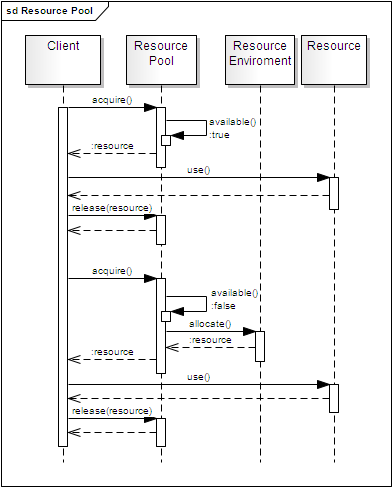
\includegraphics[width=7.75cm]{resource_pool}
\end{center}
\caption{Sequence Diagram describing how acquisition and release of resources works in a system implementing the Pooling Pattern: recycled objects are managed in a pool of resources, which allows pool clients to acquire them, and release them back to the pool when they are no longer needed.}
\label{fig:rp}
\end{figure}

To prevent the frequent acquisition and release of the aforementioned resources, our service makes use of the \emph{Pooling Pattern}~\citep{kircher2001}, in which multiple instances of one type of resource are managed in a pool.  This pool of resources allows for reuse when resource clients release resources they no longer need: released resources are put back into the pool and made available to resource clients needing them, as shown in Figure \ref{fig:rp}.

To improve efficiency, the resource pool can eagerly acquire a number of resources after its creation; then, if demand exceeds the number of available resources in pool, more resources can be lazily acquired.

There are various valid approaches to free unused resources, like those consisting of monitoring the use of a resource and controlling its lifecycle by using  strategies such as ``Least Recently Used'' or ``Least Frequently Used'', or introducing a \emph{lease} for every resource that specifies a time duration for which a resource can remain in the pool.

Relying on a resource pool results in the following improvements for our Rule-Based Machine Translation service:

\begin{description}
 \item[Performance] - by preventing repetitious acquisition and release of resources;
 \item[Predictability] - because direct acquisition of a resource from the resource enviroment can lead to unpredictable results;
 \item[Stability] - because repetitious acquisition and release of resource can increase the risk of system instability (for example, repetitious acquisition and release of memory can lead to fragmentation problems);
 \item[Scalability] - since resources can be used also in different types of translation tasks, avoiding the allocation of a complete set of resources for each different translation task (for example, translation tasks on different language pairs using different dictionaries can make use of the same transfer rules and lexical selectors);
\end{description}

\section{Results}

To evaluate the efficiency of our service, which we will refer to as {\tt apertium-service}, we compared the time it requires to compute and answer to a translation request from the Spanish language to the English language with the time required by the following systems:

\begin{itemize}
 \item {\tt apertium}, a console application implemented as a part of the Apertium project;
 \item {\tt moses}~\citep{moses}, a Statistical Machine Translation system;
 \item {\tt moses-service}, a service relying on {\tt moses}.
\end{itemize}

The translation model used by {\tt moses} and {\tt moses-service} has been trained on the well-known Europarl~\citep{europarl} corpus by using SRILM~\citep{srilm}, a toolkit for building and applying statistical language models. Language models have been then compiled into binary format using IRSTLM~\citep{irstlm}, and trained to minimize the error rate on a set of sentences from the same corpus. 

\begin{figure}[!ht]
\begin{center}
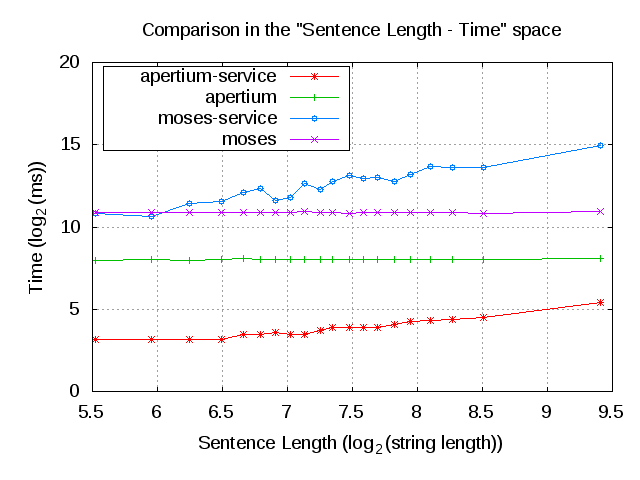
\includegraphics[width=7.75cm]{comp}
\end{center}
\caption{Comparison in the ``Sentence Length - Time'' space between {\tt apertium}, {\tt apertium-service}, {\tt moses} and {\tt moses-service}; measurements are in $log_{2}(string\ length)$ for the Sentence Length dimension and in $log_{2}(ms)$ for the Time dimension.}
\label{fig:comp}
\end{figure}

\begin{figure}[!ht]
\begin{center}
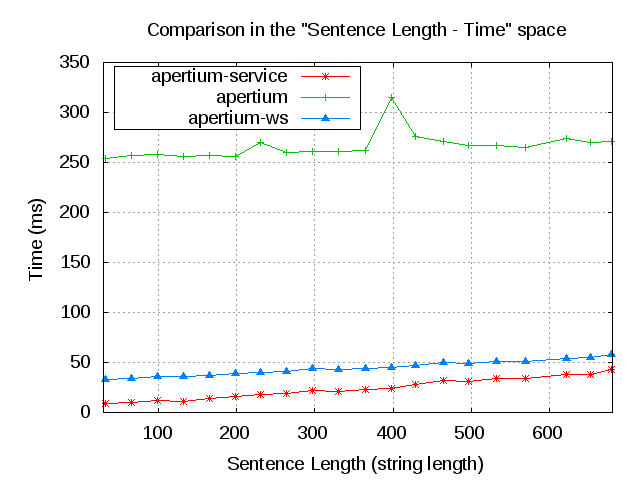
\includegraphics[width=7.75cm]{compap}
\end{center}
\caption{Comparison in the ``Sentence Length - Time'' space between {\tt apertium} and {\tt apertium-service}; measurements are in $string\ length$ for the Sentence Length dimension and in $ms$ for the Time dimension.}
\label{fig:compap}
\end{figure}


Both {\tt apertium-service} and {\tt moses-service} were accepting translation requests in XML-RPC format, and the free text used for timing all the systems was also taken from Europarl corpus. Figure \ref{fig:comp} shows the time required to translate increasingly longer sentences for all systems (values in the Time dimension are shown on a logarithmic scale), and Figure \ref{fig:compap} only for {\tt apertium-service} and {\tt apertium}.


\section{Conclusions and Future Work}

We presented {\tt apertium-service}, a Rule-Based Machine Translation service based on Apertium, a Free/Open-Source Rule-Based Machine Translation platform. It was shown to be competitive, in efficiency and scalability, with other systems based on different Machine Translation paradigms. In addition, it would be interesting to compare the results produced by {\tt apertium-service} to those produced by other Machine Translation systems and platforms also by evaluating the results they produce, for example by using some automatic evaluation metric like \emph{BLEU}~\citep{bleu} or \emph{METEOR}~\citep{meteor}, in different domains of application.


\section*{Acknowledgements}

Development for this project was funded as part of the Google Summer of Code\footnote{\url{http://code.google.com/soc/}} programme. 
Additionally, many thanks go to Jimmy O'Regan, Francis Tyers and others involved in The Apertium Project, for their constant help.


\bibliographystyle{apalike}
\bibliography{freerbmt09}

\end{document}
